\documentclass[journal,12pt,twocolumn]{IEEEtran}
%
\usepackage{setspace}
\usepackage{gensymb}
%\doublespacing
\singlespacing

%\usepackage{graphicx}
%\usepackage{amssymb}
%\usepackage{relsize}
\usepackage[cmex10]{amsmath}
%\usepackage{amsthm}
%\interdisplaylinepenalty=2500
%\savesymbol{iint}
%\usepackage{txfonts}
%\restoresymbol{TXF}{iint}
%\usepackage{wasysym}
\usepackage{amsthm}
%\usepackage{iithtlc}
\usepackage{mathrsfs}
\usepackage{txfonts}
\usepackage{stfloats}
\usepackage{bm}
\usepackage{cite}
\usepackage{cases}
\usepackage{subfig}
%\usepackage{xtab}
\usepackage{longtable}
\usepackage{multirow}
%\usepackage{algorithm}
%\usepackage{algpseudocode}
\usepackage{enumitem}
\usepackage{mathtools}
\usepackage{steinmetz}
\usepackage{tikz}
\usepackage{circuitikz}
\usepackage{verbatim}
\usepackage{tfrupee}
\usepackage[breaklinks=true]{hyperref}
%\usepackage{stmaryrd}
\usepackage{tkz-euclide} % loads  TikZ and tkz-base
%\usetkzobj{all}
\usetikzlibrary{calc,math}
\usepackage{listings}
    \usepackage{color}                                            %%
    \usepackage{array}                                            %%
    \usepackage{longtable}                                        %%
    \usepackage{calc}                                             %%
    \usepackage{multirow}                                         %%
    \usepackage{hhline}                                           %%
    \usepackage{ifthen}                                           %%
  %optionally (for landscape tables embedded in another document): %%
    \usepackage{lscape}     
\usepackage{multicol}
\usepackage{chngcntr}
%\usepackage{enumerate}

%\usepackage{wasysym}
%\newcounter{MYtempeqncnt}
\DeclareMathOperator*{\Res}{Res}
%\renewcommand{\baselinestretch}{2}
\renewcommand\thesection{\arabic{section}}
\renewcommand\thesubsection{\thesection.\arabic{subsection}}
\renewcommand\thesubsubsection{\thesubsection.\arabic{subsubsection}}

\renewcommand\thesectiondis{\arabic{section}}
\renewcommand\thesubsectiondis{\thesectiondis.\arabic{subsection}}
\renewcommand\thesubsubsectiondis{\thesubsectiondis.\arabic{subsubsection}}

% correct bad hyphenation here
\hyphenation{op-tical net-works semi-conduc-tor}
\def\inputGnumericTable{}                                 %%

\lstset{
%language=C,
frame=single, 
breaklines=true,
columns=fullflexible
}
%\lstset{
%language=tex,
%frame=single, 
%breaklines=true
%}

\begin{document}
%


\newtheorem{theorem}{Theorem}[section]
\newtheorem{problem}{Problem}
\newtheorem{proposition}{Proposition}[section]
\newtheorem{lemma}{Lemma}[section]
\newtheorem{corollary}[theorem]{Corollary}
\newtheorem{example}{Example}[section]
\newtheorem{definition}[problem]{Definition}
%\newtheorem{thm}{Theorem}[section] 
%\newtheorem{defn}[thm]{Definition}
%\newtheorem{algorithm}{Algorithm}[section]
%\newtheorem{cor}{Corollary}
\newcommand{\BEQA}{\begin{eqnarray}}
\newcommand{\EEQA}{\end{eqnarray}}
\newcommand{\define}{\stackrel{\triangle}{=}}
\bibliographystyle{IEEEtran}
%\bibliographystyle{ieeetr}
\providecommand{\mbf}{\mathbf}
\providecommand{\pr}[1]{\ensuremath{\Pr\left(#1\right)}}
\providecommand{\qfunc}[1]{\ensuremath{Q\left(#1\right)}}
\providecommand{\sbrak}[1]{\ensuremath{{}\left[#1\right]}}
\providecommand{\lsbrak}[1]{\ensuremath{{}\left[#1\right.}}
\providecommand{\rsbrak}[1]{\ensuremath{{}\left.#1\right]}}
\providecommand{\brak}[1]{\ensuremath{\left(#1\right)}}
\providecommand{\lbrak}[1]{\ensuremath{\left(#1\right.}}
\providecommand{\rbrak}[1]{\ensuremath{\left.#1\right)}}
\providecommand{\cbrak}[1]{\ensuremath{\left\{#1\right\}}}
\providecommand{\lcbrak}[1]{\ensuremath{\left\{#1\right.}}
\providecommand{\rcbrak}[1]{\ensuremath{\left.#1\right\}}}
\theoremstyle{remark}
\newtheorem{rem}{Remark}
\newcommand{\sgn}{\mathop{\mathrm{sgn}}}
\providecommand{\abs}[1]{\left\vert#1\right\vert}
\providecommand{\res}[1]{\Res\displaylimits_{#1}} 
\providecommand{\norm}[1]{\left\lVert#1\right\rVert}
%\providecommand{\norm}[1]{\lVert#1\rVert}
\providecommand{\mtx}[1]{\mathbf{#1}}
\providecommand{\mean}[1]{E\left[ #1 \right]}
\providecommand{\fourier}{\overset{\mathcal{F}}{ \rightleftharpoons}}
%\providecommand{\hilbert}{\overset{\mathcal{H}}{ \rightleftharpoons}}
\providecommand{\system}{\overset{\mathcal{H}}{ \longleftrightarrow}}
	%\newcommand{\solution}[2]{\textbf{Solution:}{#1}}
\newcommand{\solution}{\noindent \textbf{Solution: }}
\newcommand{\cosec}{\,\text{cosec}\,}
\providecommand{\dec}[2]{\ensuremath{\overset{#1}{\underset{#2}{\gtrless}}}}
\newcommand{\myvec}[1]{\ensuremath{\begin{pmatrix}#1\end{pmatrix}}}
\newcommand{\mydet}[1]{\ensuremath{\begin{vmatrix}#1\end{vmatrix}}}
%\numberwithin{equation}{section}
\numberwithin{equation}{subsection}
%\numberwithin{problem}{section}
%\numberwithin{definition}{section}
\makeatletter
\@addtoreset{figure}{problem}
\makeatother
\let\StandardTheFigure\thefigure
\let\vec\mathbf
%\renewcommand{\thefigure}{\theproblem.\arabic{figure}}
\renewcommand{\thefigure}{\theproblem}
%\setlist[enumerate,1]{before=\renewcommand\theequation{\theenumi.\arabic{equation}}
%\counterwithin{equation}{enumi}
%\renewcommand{\theequation}{\arabic{subsection}.\arabic{equation}}
\def\putbox#1#2#3{\makebox[0in][l]{\makebox[#1][l]{}\raisebox{\baselineskip}[0in][0in]{\raisebox{#2}[0in][0in]{#3}}}}
     \def\rightbox#1{\makebox[0in][r]{#1}}
     \def\centbox#1{\makebox[0in]{#1}}
     \def\topbox#1{\raisebox{-\baselineskip}[0in][0in]{#1}}
     \def\midbox#1{\raisebox{-0.5\baselineskip}[0in][0in]{#1}}
\vspace{3cm}
\title{Assignment 4: Matrix Theory}
\author{Debolena Basak\\PhD Artificial Intelligence\\ Roll No.: AI20RESCH11003}

\maketitle
\newpage
%\tableofcontents
\bigskip
\renewcommand{\thefigure}{\theenumi}
\renewcommand{\thetable}{\theenumi}

\begin{abstract}
This is a problem of a line, circle and tangent.
\end{abstract}

Download all python codes from 

\begin{lstlisting}
https://github.com/Debolena/EE5609/blob/master/Assignment_4/figure.py
\end{lstlisting}
%
and all the latex-tikz codes from 
%
\begin{lstlisting}
https://github.com/Debolena/EE5609/tree/master/Assignment_4
\end{lstlisting}
%
\section{Problem}
Find the points of intersection of the line
\begin{align}
    \label{eq1}\myvec{3 & 2}\vec x = 12
\end{align}
and the circle
\begin{align}
    \label{eq:circle} \norm{\vec{x}}^2 = 13
\end{align}
and for what values of $c$ the line
\begin{align}
    \label{tangent}\myvec{3 &2}\vec x = c 
\end{align}
touches the circle.
%\input{./chapters/problem.tex}

%In right triangle ABC, right angled at C, M is
%the mid-point of hypotenuse AB. C is joined to
%M and produced to a point D such that DM =
%CM. Point D is joined to point B. Show that
%
%\begin{enumerate}[label = (\alph*)]
%\item $\triangle  AMC  \cong   \triangle  BMD $
%\item $\triangle DBC $ is a right angle.
%\item $\triangle  DBC  \cong  \triangle  ABC $
%\item $CM = \frac{1}{2} AB$
%\end{enumerate}
%\section{Construction}
%\input{./chapters/constr.tex}
\section{Solution}
If $\vec P$ be a point on the line and $\vec n$ is the normal vector, the equation of the line can be expressed as 
\begin{align}
    & \vec n^T\brak{\vec x - \vec P}=0\\
    & \label{eq2}\implies \vec n^T \vec x = c
\end{align}
where
\begin{align}
    c= \vec n^T \vec P
\end{align}
From \brak{\ref{eq1}} and \brak{\ref{eq2}}, 
\begin{align}
     \vec n^T = \myvec{3 & 2}
\end{align}
We know,
\begin{align}
    &\vec m^T \vec n = 0\\
    &\implies \vec m^T \myvec{3 \\2} = 0\\
    &\implies \vec m ^T = \myvec{-2 & 3}
\end{align}

Now,
\begin{align}
    &\vec n^T \vec P = c \\
    &\implies \myvec{3 & 2} \vec P= 12
\end{align}

$\vec P$ can be
\begin{align}
    \myvec{4\\0}, \myvec{2\\3}, \myvec{0\\6}
\end{align}
Let us take 
\begin{align}
    \vec P =\myvec{2\\3}=\vec q
\end{align}
The circle equation:
\begin{align}
    \vec x^T \vec x + 2 \vec u^T\vec x +f=0
\end{align}
From \brak{\ref{eq:circle}},
\begin{align}
    &\vec u=\myvec{0\\0}\\
    & f=-13
\end{align}
The points of intersection of the line
\begin{align}
    L: \vec x = \vec q + \mu \vec m \quad ,\mu \in \mathbb R
\end{align}
with the conic section
\begin{align}
    \vec x^T \vec V \vec x +2\vec u^T \vec x+ f=0
\end{align}
are given by 
\begin{align}
    \label{points of intersection}\vec x_i = \vec q + \mu _i \vec m
\end{align}
where,

\begin{multline}
\mu_i = \frac{1}
{
\vec{m}^T\vec{V}\vec{m}
}
\lbrak{-\vec{m}^T\brak{\vec{V}\vec{q}+\vec{u}}}
\\
\pm
{\small
\rbrak{\sqrt{
\sbrak{
\vec{m}^T\brak{\vec{V}\vec{q}+\vec{u}}
}^2
-
\brak
{
\vec{q}^T\vec{V}\vec{q} + 2\vec{u}^T\vec{q} +f
}
\brak{\vec{m}^T\vec{V}\vec{m}}
}
}
}
\end{multline}
For circle,
\begin{align}
    &\vec V = \vec I\\ 
    & \therefore \mu_i = \frac{1}{13}\lbrak{-5 \pm \rbrak{\sqrt{25- \brak{13-13}13}
    }
    }\\
    & = \frac{1}{13}\brak{-5 \pm 5}\\
    & = 0, -\frac{10}{13}
\end{align}
Using \brak{\ref{points of intersection}}, the points of intersection are given by
\begin{align}
    \vec x = \myvec{2\\3} , \myvec{\frac{46}{13}\\ \frac{9}{13}}
\end{align}
Points of contact are given by
\begin{align}
    \vec q = \vec V^{-1} \brak{\kappa \vec n - \vec u}\\
    \kappa = \pm \sqrt{\frac{\vec u^T \vec V^{-1} \vec u -f}{\vec n^T \vec V^{-1} \vec n}}
\end{align}
Since for circle,
\begin{align}
    &\vec V= \vec I\\
    &\therefore \vec V^{-1} = \vec I \quad \because \vec I^{-1}
    = \vec I\\
    &\therefore \kappa =\pm  \sqrt{\frac{-f}{\vec n^T \vec n}}\quad\because \vec u^T\vec u= 0\\
    & = \pm \sqrt{\frac{13}{\myvec{3 & 2}\myvec{3\\2}}}\\
    & = \pm \sqrt{\frac{13}{13}}\\
    & = \pm 1\\
    &\therefore \vec q = \pm 1\myvec{3\\2}\\
    & = \myvec{3\\2}, \myvec{-3\\-2}
\end{align}
From \brak{\ref{tangent}},
\begin{align}
    c = \myvec{3 & 2}\myvec{3\\2} = 13, \\ \myvec{3&2}\myvec{-3\\-2}=-13
\end{align}
The line \brak{\ref{tangent}} touches the circle for $c = 13, -13$.

\begin{figure}[!]
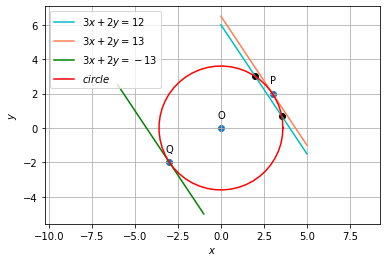
\includegraphics[width=1\columnwidth]{figure.png}
\caption{Circle with tangent and intersection lines}
\end{figure}

%\vspace{5mm} 

%\input{./chapters/solution.tex}
%\subsection{Sol.a)}
%\input{./chapters/sol_a.tex}
%\subsection{Sol.b)}
%\input{./chapters/sol_b.tex}
%\subsection{Sol.c)}
%\input{./chapters/sol_c.tex}
%\subsection{Sol.d)}
%\input{chapters/sol_d.tex}
\end{document}
